
% commentaires



%----------------------------------------------------------------------------------------
%	PACKAGES AND OTHER DOCUMENT CONFIGURATIONS
%----------------------------------------------------------------------------------------

%\documentclass[]{article}

%\documentclass[11pt,fleqn]{book} % Default font size and left-justified equations
%\documentclass[]{book}
\documentclass[oneside]{book}
%\documentclass[twoside]{scrbook}
%\documentclass[oneside]{scrbook}
%\documentclass[oneside]{report}


%\usepackage[top=3cm,bottom=3cm,left=3.2cm,right=3.2cm,headsep=10pt,a4paper]{geometry} % Page margins
%\usepackage[top=3cm,bottom=3cm,left=3.2cm,right=2.2cm,headsep=60pt,a4paper]{geometry} % Page margins
%https://fr.sharelatex.com/learn/Page_size_and_margins
\usepackage[top=0.5cm,bottom=1.5cm,left=1cm,right=1cm,headsep=60pt,a5paper,landscape]{geometry} % Page margins

%\usepackage[latin1]{inputenc} % KO
\usepackage[francais]{babel}


\usepackage{xcolor} % Required for specifying colors by name
\definecolor{ocre}{RGB}{243,102,25} % Define the orange color used for highlighting throughout the book

% Index
\usepackage{calc} % For simpler calculation - used for spacing the index letter headings correctly
\usepackage{makeidx} % Required to make an index
\makeindex % Tells LaTeX to create the files required for indexing

\renewcommand{\thesection}{\arabic{section}} % pb numerotation avec chapter, evite le 0.1

\renewcommand{\contentsname}{Sommaire}
%\renewcommand{\chaptername}{Chapitre}
\renewcommand{\chaptername}{}
% voir : https://en.wikibooks.org/wiki/LaTeX/Customizing_Page_Headers_and_Footers

\renewcommand{\floatpagefraction}{.8} % influence le nombre d'image dans la page
%https://tex.stackexchange.com/questions/192622/is-there-a-value-for-textfraction-and-totalnumber-floatpagefraction-that-i-s

% Placement des images
% voir http://www.andy-roberts.net/writing/latex/floats_figures_captions



%----------------------------------------------------------------------------------------
% header footer
%----------------------------------------------------------------------------------------

\usepackage{fancyhdr}

\fancypagestyle{plain}{
	\fancyhf{}
	\fancyhead[L]{
\includegraphics[width=0.15000\textwidth]{../screenshots/logo.237.135.png}}
	\fancyfoot[C]{\footnotesize https://e-carnet-maternelle.jimdofree.com/   -   support@tr-esolutions.com - Page \thepage\ }
}


\pagestyle{fancy}
\chead{\raisebox{\baselineskip}{%
  
\includegraphics[width=1.5cm,height=1.5cm,keepaspectratio]{../screenshots/logo.237.135.png}}}
%\rfoot{\footnotesize support@tr-esolutions.com - Page \thepage\ of \pageref{LastPage}}
\cfoot{\footnotesize https://e-carnet-maternelle.jimdofree.com/   -   support@tr-esolutions.com - Page \thepage\ }

%\fancypagestyle{plain}{%
%  \renewcommand{\headrulewidth}{0pt}%
%  \fancyhf{}%
%  \fancyfoot[C]{\footnotesize support@tr-esolutions.com - Page \thepage\ of \pageref{LastPage}}%
%}

%\pagestyle{fancy}
%\fancyhf{}
%\rhead{Share\LaTeX}
%\lhead{Guides and tutorials}
%\lfoot{support@tr-esolutions.com}


%----------------------------------------------------------------------------------------
% https://www.sharelatex.com/learn/Paragraph_formatting
%----------------------------------------------------------------------------------------

\usepackage{lmodern}
\usepackage{amssymb,amsmath}
\usepackage{ifxetex,ifluatex}
%\usepackage{fixltx2e} % provides \textsubscript
\ifnum 0\ifxetex 1\fi\ifluatex 1\fi=0 % if pdftex
  \usepackage[T1]{fontenc}
  \usepackage[utf8]{inputenc}
\else % if luatex or xelatex
  \ifxetex
    \usepackage{mathspec}
  \else
    \usepackage{fontspec}
  \fi
  \defaultfontfeatures{Ligatures=TeX,Scale=MatchLowercase}
\fi
% use upquote if available, for straight quotes in verbatim environments
\IfFileExists{upquote.sty}{\usepackage{upquote}}{}
% use microtype if available
\IfFileExists{microtype.sty}{%
\usepackage[]{microtype}
\UseMicrotypeSet[protrusion]{basicmath} % disable protrusion for tt fonts
}{}
\PassOptionsToPackage{hyphens}{url} % url is loaded by hyperref
\usepackage[unicode=true]{hyperref}
\hypersetup{
            pdftitle={Documentation application Ecm référentiel builder pour e-carnet de maternelle},
            pdfauthor={support@tr-esolutions.com},
            pdfborder={0 0 0},
            breaklinks=true}
\urlstyle{same}  % don't use monospace font for urls



\usepackage{graphicx,grffile}

% save the meaning of \includegraphics
% redefine to auto resize
%\LetLtxMacro\latexincludegraphics\includegraphics
%\renewcommand{\includegraphics}[2][]{\includegraphics[width=5cm]{#2}}
%KO
%\renewcommand{\includegraphics}[2][]{\includegraphics[width=0.50000\textwidth]{#2}}

\makeatletter
\def\maxwidth{\ifdim\Gin@nat@width>\linewidth\linewidth\else\Gin@nat@width\fi}
\def\maxwidth{0.50000\textwidth}
\def\maxheight{\ifdim\Gin@nat@height>\textheight\textheight\else\Gin@nat@height\fi}
\makeatother

% Scale images if necessary, so that they will not overflow the page
% margins by default, and it is still possible to overwrite the defaults
% using explicit options in \includegraphics[width, height, ...]{}
\setkeys{Gin}{width=\maxwidth,height=\maxheight,keepaspectratio}



\IfFileExists{parskip.sty}{%
\usepackage{parskip}
}{% else
\setlength{\parindent}{0pt}
\setlength{\parskip}{6pt plus 2pt minus 1pt}
}

\setlength{\emergencystretch}{3em}  % prevent overfull lines

\providecommand{\tightlist}{%
  \setlength{\itemsep}{0pt}\setlength{\parskip}{0pt}}

\setcounter{secnumdepth}{5}

% Redefines (sub)paragraphs to behave more like sections
\ifx\paragraph\undefined\else
\let\oldparagraph\paragraph
\renewcommand{\paragraph}[1]{\oldparagraph{#1}\mbox{}}
\fi
\ifx\subparagraph\undefined\else
\let\oldsubparagraph\subparagraph
\renewcommand{\subparagraph}[1]{\oldsubparagraph{#1}\mbox{}}
\fi


\usepackage{float} % IMPORTANT sur le placement des images
% set default figure placement to htbp
%\makeatletter
%\def\fps@figure{htbp}
%\makeatother

\makeatletter
\def\fps@figure{H} % IMPORTANT sur le placement des images H = HERE : en place, dans le flow.
\makeatother




\title{Documentation application Ecm référentiel builder pour e-carnet de
maternelle}


\author{support@tr-esolutions.com}

\providecommand{\institute}[1]{}
\institute{TR e-solutions}

\date{Version 1.0.3 du 18 novembre 2019}

\begin{document}


\vbox{
    \centering
    
\includegraphics{../screenshots/logo.237.135.png}
    \maketitle %this typesets the contents of \title, \author and \date
}







%----------------------------------------------------------------------------------------
%	 TOC
%----------------------------------------------------------------------------------------

{
\setcounter{tocdepth}{5}
\tableofcontents
}


%----------------------------------------------------------------------------------------
%	 LOT
%----------------------------------------------------------------------------------------


%----------------------------------------------------------------------------------------
%	 LOF
%----------------------------------------------------------------------------------------


\listoffigures

\chapter{e-carnet de maternelle}

%----------------------------------------------------------------------------------------
%	 BODY
%----------------------------------------------------------------------------------------

\hypertarget{e-carnet-maternelle-ruxe9fuxe9rentiel-builder}{%
\section{E-carnet maternelle référentiel
builder}\label{e-carnet-maternelle-ruxe9fuxe9rentiel-builder}}

\begin{figure}
\centering

\includegraphics{./screenshots/logo.237.135.png}
\caption{Icone de l'application}
\end{figure}

\hypertarget{pruxe9sentation-de-lapplication}{%
\subsection{Présentation de
l'application}\label{pruxe9sentation-de-lapplication}}

L'application \textbf{\emph{Ecm referentiel builder}} est une
application compagon de l'application e-carnet de maternelle.

Elle permet de produire un fichier utilisable uniquement par
l'application e-carnet de maternelle (version \textgreater{} 1.8.0v93,
publiée à partir du 17 novembre 2019).

Ce fichier ainsi produit contient l'arborescence d'un référentiel de
compétences personnalisé.

Pour mémoire,

Le e-carnet maternelle\index{e-carnet maternelle} est une application
gratuite pour les enseignants et les élèves de cycle 1.

Elle permet de saisir et stocker instantanément tous types de documents
(image, audio, vidéo, texte) pour chaque élève de la classe.

Ces traces\index{Traces} sont associés aux attendus et observables
établis par le Ministère de l'Éducation Nationale\index{Ministère}.

Un commentaire de l'élève ainsi qu'un commentaire de l'enseignant
peuvent être ajoutés.

Les carnets de suivi sont générés automatiquement et envoyés par mail
aux parents\index{Parents}.

Ce n'est pas un carnet de compétences, on prend l'élève au niveau qui
est le sien, il est la référence, et on constate avec lui ses progrès au
cours du temps. Conformément aux textes officiels, il n'y a pas de code
de ``notation''.

Pour plus d'informations, voir le site web
\href{https://e-carnet-maternelle.jimdofree.com}{e-carnet-maternelle}.

\hypertarget{ruxe9fuxe9rence}{%
\subsection{Référence}\label{ruxe9fuxe9rence}}

L'application e-carnet-de-maternelle s'appuye et mettre en oeuvre le
référentiel\index{Référentiel} décrit dans ce document
Eduscol\index{Eduscol} qui constitue la version d'origine de ce
référentiel.

Référence éducation nationale :
\href{http://eduscol.education.fr/cid97131/suivi-et-evaluation-a-l-ecole-maternelle.html}{Le
carnet de suivi des apprentissages en maternelle}

\begin{figure}
\centering
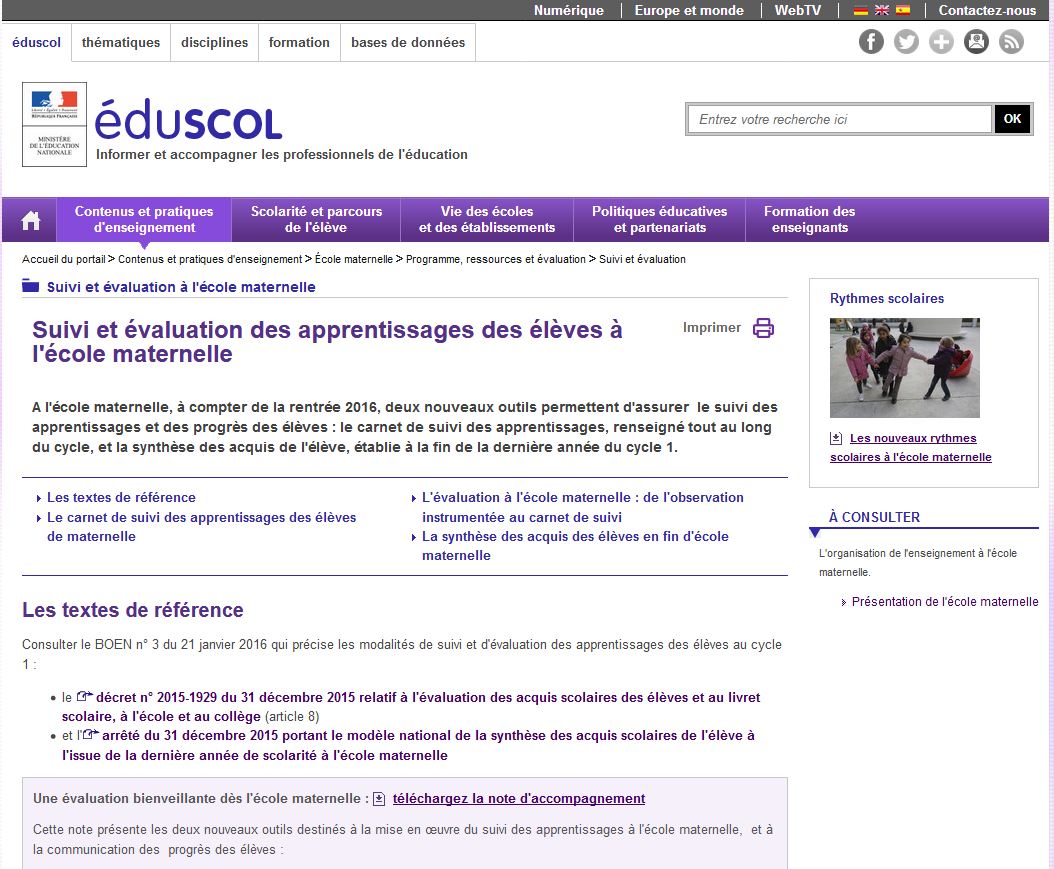
\includegraphics{./screenshots/2018-01-27-18-00-46.png}
\caption{Le carnet de suivi des apprentissages en maternelle}
\end{figure}

\hypertarget{avertissement}{%
\subsection{Avertissement}\label{avertissement}}

L'utilisation d'un référentiel différent de celui proposé par
l'Education Nationale n'est pas recommandée pour les établissements
francophones qui mettent en oeuvre le programme officiel.

Elle évolue régulièrement.

\hypertarget{en-savoir-plus-le-site-web}{%
\subsection{En savoir plus : le site
web}\label{en-savoir-plus-le-site-web}}

Retrouvez la dernière version sur le \index{Site web} de l'application :

\href{https://e-carnet-maternelle.jimdofree.com/}{e-carnet-maternelle.jimdofree.com}

\begin{figure}
\centering
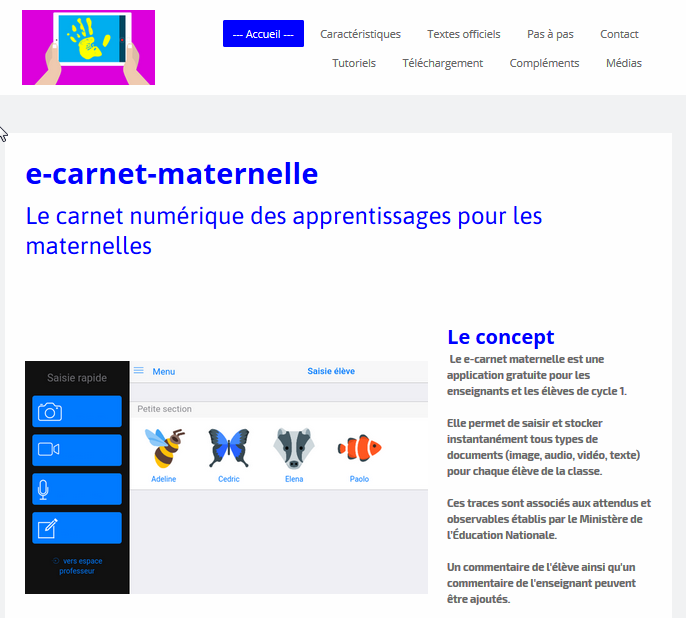
\includegraphics{./screenshots/2018-02-06-06-39-29.png}
\caption{Le site web}
\end{figure}

Découvrez les tutoriels\index{Tutoriels} !

\begin{figure}
\centering
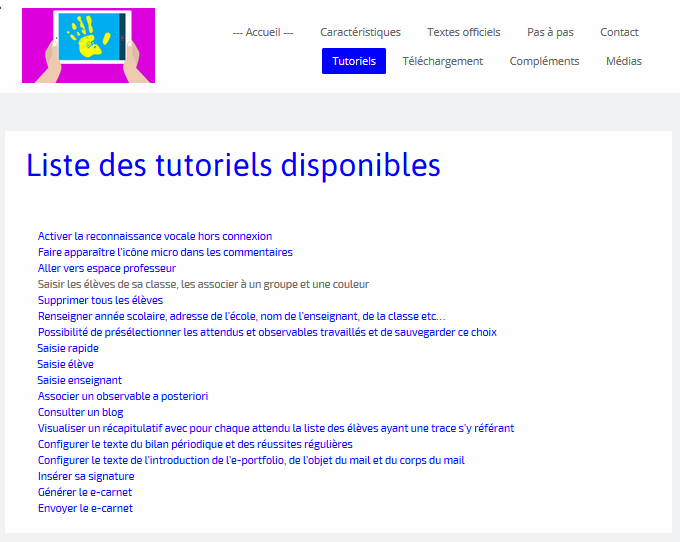
\includegraphics{./screenshots/2018-02-06-06-40-51.png}
\caption{Les tutoriels}
\end{figure}

Consignes de téléchargement\index{Téléchargement} de cette documentation
et de l'application :

\begin{figure}
\centering
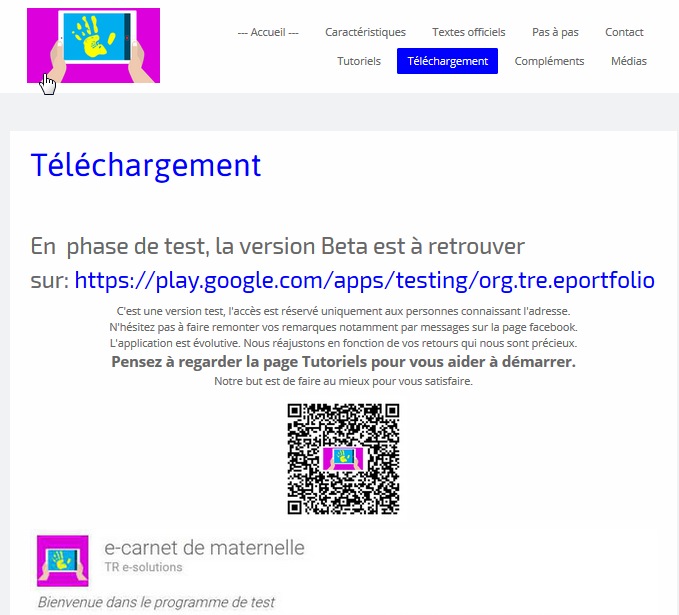
\includegraphics{./screenshots/2018-02-06-06-41-57.png}
\caption{Téléchargement}
\end{figure}

\hypertarget{nouveautuxe9s}{%
\section{Nouveautés}\label{nouveautuxe9s}}

\hypertarget{version-1.0.3-du-17-novembre-2019}{%
\subsection{Version 1.0.3 du 17 novembre
2019}\label{version-1.0.3-du-17-novembre-2019}}

C'est la première version publiée.

\hypertarget{parcours-professeur}{%
\section{Parcours professeur}\label{parcours-professeur}}

\hypertarget{suxe9curituxe9-donnuxe9es-personnelles-rgpd}{%
\section{\texorpdfstring{Sécurité, données personnelles,
RGPD\index{Sécurité}\index{Données personnelles}\index{RGPD}}{Sécurité, données personnelles, RGPD}}\label{suxe9curituxe9-donnuxe9es-personnelles-rgpd}}

L'application est enregistrée à la CNIL\index{CNIL} sous le numéro :
2119239 du 14 novembre 2017.

Ces sujets sont abordés dans un document à part, disponible sur demande
à l'adresse mail : \url{support@tr-esolutions.com}

\hypertarget{cruxe9dits}{%
\section{\texorpdfstring{Crédits\index{Crédits}}{Crédits}}\label{cruxe9dits}}

L'application Ecm Référentiel builder utilise de multiples composants
logiciels open source\index{Open source} pour la plupart :

\begin{itemize}
\item
  \href{}{Blockly}
\item
  \href{https://developer.android.com/studio/index.html}{AndroidSdK}
\item
  \href{https://developer.android.com/studio/index.html}{AndroidStudio}
\item
  \href{https://code.visualstudio.com/}{VisualStudio Code}
\item
  \href{https://cordova.apache.org/}{cordova}
\item
  \href{https://cordova.apache.org/plugins/}{cordova plugins}
\item
  \href{https://framework7.io/}{Framework7}
\item
  \href{https://nodejs.org/}{nodeJS}
\item
  \href{https://gulpjs.com/}{Gulp}
\item
  \href{https://www.npmjs.com/}{npm}
\item
  \href{https://en.wikipedia.org/wiki/Markdown}{markdown}
\item
  \href{https://pandoc.org/}{Pandoc}
\item
  \href{https://www.tug.org/texworks/}{TexWorks}
\item
  \href{https://miktex.org/}{MikTex}
\item
  \href{https://framagit.org/}{FramaGit}
\item
  script JS :
\end{itemize}

\hypertarget{evolutions-uxe0-venir}{%
\section{\texorpdfstring{Evolutions à
venir\index{Evolutions}}{Evolutions à venir}}\label{evolutions-uxe0-venir}}

N'hésitez pas à communiquer vos souhaits et commentaires. Quel que soit
le moyen de votre choix.

\hypertarget{bugs-identifiuxe9s-uxe0-corriger}{%
\section{Bugs identifiés à
corriger}\label{bugs-identifiuxe9s-uxe0-corriger}}

\begin{itemize}
\tightlist
\item
  La mise en forme de la fiche élève en mode édition n'est pas homogène.
\item
  Il arrive que la vignette de l'élève ne s'affiche pas dans le
  e-carnet. Palliatif : recommencer ``Générer e-carnet''.
\end{itemize}

%----------------------------------------------------------------------------------------
%	 END of BODY
%----------------------------------------------------------------------------------------



%----------------------------------------------------------------------------------------
%	INDEX
%----------------------------------------------------------------------------------------

\cleardoublepage
\setlength{\columnsep}{0.75cm}
%\addcontentsline{toc}{chapter}{\textcolor{ocre}{Index}}
\addcontentsline{toc}{Partie}{Index}
\printindex{}

\end{document}
